\documentclass[a4paper,pagesizefontsize=12pt]{scrartcl}
\usepackage[ngerman]{babel}
\usepackage[utf8]{inputenc}
\usepackage[T1]{fontenc}
\usepackage{caption}
\usepackage[babel,german=quotes]{csquotes}
\usepackage{setspace}
\usepackage{xcolor}
\usepackage[linkbordercolor=blue, urlbordercolor=blue]{hyperref}
\usepackage{graphicx} 
\usepackage{float}
%\usepackage[left=30mm,right=20mm,top=25mm,bottom=25mm]{geometry}
\usepackage{mathcomp}
\usepackage{amsthm}
\usepackage{amsmath}
\usepackage{amssymb}

\newcommand\R{\mathbb{R}}
\newcommand\N{\mathbb{N}}
\newcommand\Z{\mathbb{Z}}
\newcommand\C{\mathbb{C}}

\newtheorem{satz}{Satz}
\newtheorem{lem}{Lemma}
\newtheorem{prop}{Proposition}
\newtheorem*{prop*}{Proposition}
\newtheorem{kor}{Korollar}


\theoremstyle{definition}
\newtheorem*{defi*}{Definition}
\newtheorem{defi}{Definition}
\newtheorem{bsp}{Beispiel}
\newtheorem*{bsp*}{Beispiel}

\theoremstyle{remark}
\newtheorem{bem}{Bemerkung}
\newtheorem*{bem*}{Bemerkung}




\begin{document}

\section* {Knotentheorie - Stefan Knoblauch}

\begin{enumerate}
\item Knoten
\item Äquivalenz von Knoten
\item Fundamentalgruppe
\end{enumerate}

\begin{bsp*}
\begin{figure}[H]
\center
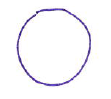
\includegraphics[trim = 0mm 2mm 0mm 0px,clip, width=0.15\linewidth]{Unknoten}
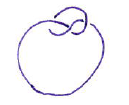
\includegraphics[width=0.16\linewidth]{Kleeblattknoten}
\caption*{Unknoten und Kleeblattknoten}
\end{figure}
\end{bsp*}

\begin{section}{Knoten}

\begin{defi}
Ein \textit{Knoten} ist eine einfache, geschlossene Kurve, also
\begin{itemize}
\item $K:[0,1] \longrightarrow \R^{3} $ stetig,
\item $K(0) = K(1)$ und
\item $K(x) =K(y) \Rightarrow (x=y)\vee(x=0 \wedge y=1)\vee(x=1 \wedge y=1)$
\end{itemize}
\end{defi}
\vspace{0.2cm}

Problem: 
\begin{figure}[H]
\center
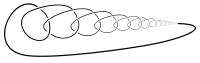
\includegraphics[width=0.4\linewidth]{WilderKnoten}
\caption* {\enquote{WilderKnoten}  \href{http://de.wikipedia.org/wiki/Datei:Wild\_knot.svg}{Quelle: Wikipedia}}
\end{figure}
\vspace{0.2cm}

Deshalb zusätzliche Forderung für Knoten:
\begin{defi}
Ein \textit{Knoten} ist eine einfache, geschlossene Kurve, also
\begin{itemize}
\item $K:[0,1] \longrightarrow \R^{3} $ stetig,
\item $K(0) = K(1)$,
\item $K(x) =K(y) \Rightarrow (x=y)\vee(x=0 \wedge y=1)\vee(x=1 \wedge y=1)$ und
\item $K$ ist stetig differnzierbar auf $[0,1]$
\end{itemize}
\end{defi}

\begin{defi}
Sei $(p_1, \dots, p_n)\ mit\ p_i \in \R^3 \ \forall i\in \{1, \dots, n\}$, dann heißt die Vereinigung von den Strecken $[p_1, p_2], [p_2,p_3], \dots, [p_{n-1}, p_n], [p_n, p_1]$ \textit{geschlossener Polygonzug}, wobei \\ $[p_i,p_{i+1}] := \{p_i + (p_{i+1}-p_i)\lambda \  |\  \lambda \in [0,1]\}$.
Ein \textit{Knoten} ist ein einfacher(d.h., dass alle Ecken von einander verschieden sind und 2 verschiedene Kanten nur in Ecken den selben Wert annehmen), geschlossener Polygonzug.
\end{defi}

\begin{figure}[H]
\center
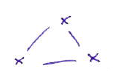
\includegraphics[width=0.22\linewidth]{UnknotenPolygon}
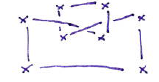
\includegraphics[width=0.23\linewidth]{KleeblattknotenPolygon}
\caption*{Unknoten und Kleeblattknoten als Polygonzüge}
\end{figure}
\vspace{0.3cm}

\begin{defi}
Eine \textit{Verschlingung} ist eine endliche Vereinigung von einfachen, geschlossenen Polygonzügen. Ein \textit{Knoten} ist die Vereingung von genau einer Verschlingung.
\end{defi}

\begin{figure}[H]
\center
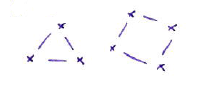
\includegraphics[width=0.35\linewidth]{Verschlingung}
\caption*{Triviale Verschlingung}
\end{figure}
\vspace{0.3cm}
\end{section}

\begin{section}{Äquivalenz}

\begin{figure}[H]
\center
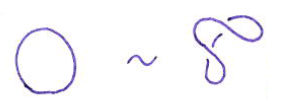
\includegraphics[width=0.4\linewidth]{Aequivalenz}
\caption* {Zwei Unknoten}
\end{figure}

\begin{defi}
Seien $(X,d_1)$ und $(Y,d_2)$ metrische Räume und $f,g: X\longrightarrow Y$ Abbildungen, dann ist eine stetige Abbildung  $h: X\times [0,1]\longrightarrow Y$ mit $h(-,0)=f\  \wedge \ h(-,1)=g$ eine \textit{Homotopie} zwischen $f$ und $g$.
\end{defi}

\begin{bsp*}
\begin{align*}
&f:\R\rightarrow \R\ ,\ x\mapsto x 
\\&g:\R\rightarrow \R\ ,\ x\mapsto 2x+1
\\&h:\R\times[0,1] \rightarrow \R\ , \ (x,t)\mapsto(1+t)x+t
\end{align*}
\begin{figure}[H]
\center
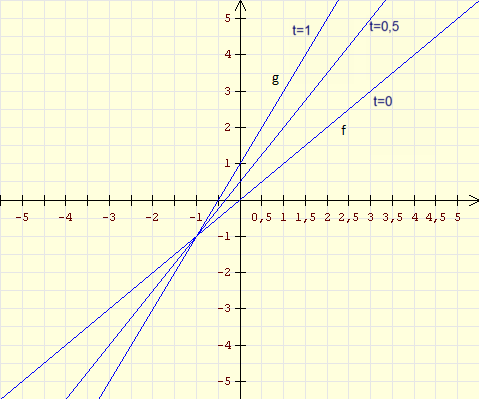
\includegraphics[width=0.7\linewidth]{Homotopie}
\caption*{\href{http://www.arndt-bruenner.de/mathe/java/plotter.htm}{Quelle: Arndt-Brünner}}
\end{figure}
\end{bsp*}

\begin{defi}
Zwei Knoten $K,J : [0,1]\longrightarrow \{R^3$ heißen \textit{äquivalent}, falls
\begin{displaymath}
K\sim J\ :\Leftrightarrow \ \exists H : [0,1] \times [0,1] \rightarrow \R^3\ mit \\
\left\{\begin{array}{l} \left. \begin{array}{l}
H(-,0) = K\qquad \qquad \qquad\qquad \\
H(-,1)=K\\
\end{array} \right\} \text{H ist Homotopie}
\\ \, \   H(-,t)\text{ ist Knoten}\ \forall t \in[0,1]
\end{array}\right.
\end{displaymath}
\end{defi}

Dies definiert eine Äquivlanzrelation, da
\begin{itemize}
\item \textbf{Reflexivität}
\\ $K\sim K$ mit $H:[0,1]\times [0,1] \longrightarrow \R^3$, $(x,-) \mapsto K(x)$
\item \textbf{Symmetrie}
\\ $K\stackrel{H_{alt}}{\sim}J \Rightarrow J\stackrel{H_{neu}}{\sim}K$ \qquad mit $H_{neu}(x.t) := H_{alt}(x,1-t)$
\item \textbf{Transitivität}
\\ $K\stackrel{H_{1}}{\sim}J$ und $J\stackrel{H_{2}}{\sim}L \Rightarrow K\stackrel{H}{\sim}L$ \qquad mit $H(x,t) :=
\begin{cases} 
H_1(x,2t) &\mbox{für } 0\leq t \leq 0,5
\\H_2(x,2t-1) & \mbox{für } 0,5 < t \leq 1
\end{cases} $
\end{itemize}

Dazu äquivalent:
\begin{defi}
\begin{displaymath}
K\sim J\ :\Leftrightarrow \ \exists H : [0,1] \times [0,1] \rightarrow \R^3\ mit \\
\left\{\begin{array}{l} 
H(-,0) = \mathrm{id} \\
H(K(x),1)=J(x)\ \forall x\in [0,1]\\
\underbrace{H(-,t)\text{ ist bijektiv, stetig und }H^{-1}(-,t) \text{ ist stetig}}_{\text{H ist Homömorphismus}}
\end{array}\right.
\end{displaymath}
\end{defi}

\begin{bsp*}
$K(\lambda) := \begin{pmatrix}0\\\cos (2\pi \lambda)\\ \sin(2\pi \lambda) \end{pmatrix}$, $J(\lambda) := \begin{pmatrix}\cos (2\pi \lambda)\\ 0\\ \sin(2\pi \lambda) \end{pmatrix}$
\begin{figure}[H]
\center
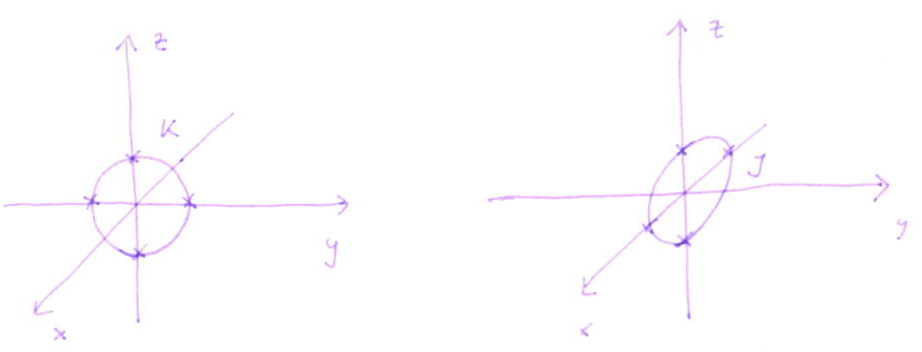
\includegraphics[width=0.7\linewidth]{Kreise}
\end{figure}
$H(\begin{pmatrix}x\\y\\ z \end{pmatrix},t) := 
\begin{pmatrix}
&\cos (\frac{\pi}{2} t) & \sin (\frac{\pi}{2} t) & 0 \\
&-\sin (\frac{\pi}{2} t) & \cos (\frac{\pi}{2} t) & 0 \\
& 0 & 0 & 1
\end{pmatrix} 
\begin{pmatrix}
x\\y\\z
\end{pmatrix}$, dann: \vspace{0.4 cm} \\ 
$H(K(x),1) = \begin{pmatrix}
0 & 1 & 0 \\
-1 & 0 & 0 \\
0 & 0 & 1
\end{pmatrix} K(x) = \begin{pmatrix}\cos (2\pi \lambda)\\ 0\\ \sin(2\pi \lambda) \end{pmatrix} = J(x)$
\end{bsp*}
\vspace{0.2cm}

\begin{defi}
Die Funktion $P: \R ^3 \longrightarrow \R ^2,\ \begin{pmatrix}
x\\y\\z
\end{pmatrix} \mapsto \begin{pmatrix}
x\\y
\end{pmatrix}$ ist die Projektion auf die ersten beiden Komponenten.
\end{defi}
\vspace{0.2cm}

\begin{defi}
Das Bild dieser Projektion $P$ heißt \textit{reguläre Position}, falls
\begin{itemize}
\item je nur 2 Punkte des Knotens das selbe Bild haben und
\item kein Eckpunkt auf einen Punkt abgebildet wird, auf den noch ein anderer Punkt abgebildet wurde.
\end{itemize}
\end{defi}
\end{section}

\begin{section}{Fundamentalgruppe}

\begin{defi}
Seien $(X,d)$ metrischer Raum und $p \in X$, dann ist\\ $\Omega(X,p) :=\ $\{Kurven $K:[0,1]\rightarrow V$ mit $K(0)=K(1)=p\}$ die Fundamentalgruppe von p in X.
\end{defi}

\begin{defi}
Seien $f,g : [0,1] \longrightarrow X$ Kurven, dann\\
$(f\star g)(t) :=
\begin{cases} 
f(2t) &\mbox{für } 0\leq t \leq 0,5\\
g(2t-1) & \mbox{für } 0,5 < t \leq 1
\end{cases} $
\end{defi}
\vspace{0.3cm}

Achtung, diese Komposition ist nicht kommutativ!
\begin{bsp*}
\ \\
\begin{figure}[H]
\center
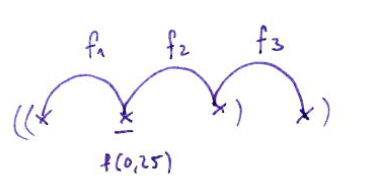
\includegraphics[width=0.5\linewidth]{Komposition1}
\caption*{$f=(f_1 \star f_2)\star f_3$}
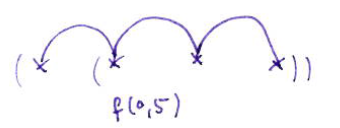
\includegraphics[width=0.5\linewidth]{Komposition2}
\caption*{$f=f_1 \star (f_2\star f_3)$}
\end{figure}
\end{bsp*}
\vspace{0.1cm}

\begin{defi}
$K$ homotop zu $J$ mit festem Endpunkt p\\
$:\Leftrightarrow \exists H : [0,0] \times [0,1] \rightarrow X$ stetig mit $\left\{\begin{array}{l} 
H(-,0) = K \\
H(K(x),1)=J\\
H(0,t)=H(1,t)=p\ \forall t \in[0,1]
\end{array}\right.$
\end{defi}
\vspace{0.2cm}

\begin{defi}
Sei $\pi_1(X,p) := \Omega(X,p)/_{\sim}$ die Projektion auf die Äquivalenzklasse $[p] $, dann
\begin{displaymath}
\begin{array}{rl} 
\star : \pi_1(X,p) \times \pi_1(X,p) &\rightarrow \pi_1(X,p) \\
([a],[b]) & \mapsto [a\circ b]
\end{array}
\end{displaymath}
\end{defi}

\begin{prop*}
Seien $a,a',b,b' \in \Omega (X,p)$ und gelte $a\stackrel{H_{1}}{\sim} a'$ und $b\stackrel{H_{2}}{\sim} b'$, dann 
\\$a\circ b\stackrel{H}{\sim} a'\circ b'$ mit $H: [0,1]\times[0,1] \rightarrow X,\ H(-,t) := H_1(-,t)\star H_2(-,t)$
\end{prop*}
\vspace{0.2cm}

\begin{bsp*}Fundamentalgruppe von 
\begin{itemize}
\item $  \R ^3\qquad \, \qquad  \pi_1(\R ^3,1) = \{0\}$
\item $\R ^3 \backslash \{0\} \qquad  \pi_1(\R ^3\backslash\{0\},1)= \{0\}$
\item $\R ^2 \backslash \{0\} \qquad  \pi_1(\R ^2\backslash\{0\},1)= \Z$
\item 
\begin{figure}[H]
\center
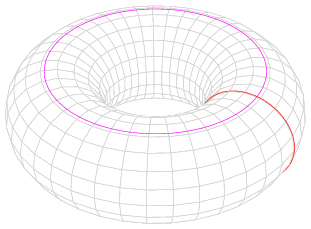
\includegraphics[width=0.25\linewidth]{Torus}
\caption*{$\Z \times \Z$ }
\caption*{\href{http://scienceblogs.de/mathlog/wp-content/blogs.dir/18/files/2012/06/i-7dd715a5c3485c289f4b74c61c3993ac-Torus\_cycles.png}{Quelle: scienceblogs.de}}
\end{figure}
\item 
\begin{figure}[H]
\center
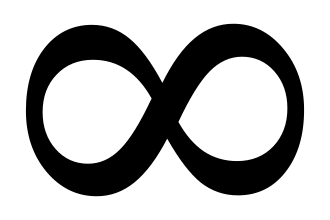
\includegraphics[width=0.25\linewidth]{Unendlich}
\caption*{$\Z \star \Z$ }
\caption*{\href{http://www.mediamanual.at/mediamanual/workshop/visual/image/unendlich.png}{Quelle: mediamanual.at}}
\end{figure}
\item 
\begin{figure}[H]
\center
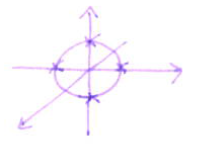
\includegraphics[width=0.35\linewidth]{Kreis}
\caption*{$\Z$}
\end{figure}
\end{itemize}
\end{bsp*}

\begin{bem*}
$\pi_1$ ist ein \textit{Funktor} von der Kategorie der (punktierten) topologischen Räume in die Kategorie der Gruppe. Neben anderen Funktoren (Homologie, Kohomologie,...) bildet er eine fundamentale Verbindung zwischen Topologie und Algebra.
\end{bem*}

\end{section}
\end{document}